\documentclass[12pt,a4paper]{article}

\usepackage[utf8]{inputenc}
\usepackage[T1]{fontenc}
\usepackage[brazil]{babel}
\usepackage{graphicx}
\usepackage{geometry}
\usepackage{amsmath}
\usepackage{hyperref}
\usepackage{float}
\usepackage{subcaption}
\usepackage{booktabs}
\usepackage{parskip}
\usepackage{microtype}
\usepackage{xcolor}
\usepackage{listings}

\geometry{
  a4paper,
  top=2.5cm, bottom=2.5cm,
  left=3cm,  right=2.5cm
}

\hypersetup{
  colorlinks=true,
  linkcolor=black,
  urlcolor=blue
}

\lstset{
  basicstyle=\ttfamily\small,
  breaklines=true,
  frame=single,
  language=Python,
  keywordstyle=\color{blue},
  commentstyle=\color{gray},
  stringstyle=\color{orange},
}

% ------------------------------------------------------------------
\title{
  \textbf{INF2608 -- Fundamentos da Computação Gráfica}\\[0.4em]
  \large Projeto 1: Algoritmo de Traçado de Raio
}
\author{Lucca Rocha}
\date{10 de maio de 2026}
% ------------------------------------------------------------------

\begin{document}

\maketitle
\tableofcontents
\newpage

% ==================================================================
\section{Introdução}
% ==================================================================

Este relatório descreve a implementação de um motor de traçado de raios
(\textit{ray tracer}) desenvolvido em Python como parte do Projeto 1 da
disciplina INF2608 -- Fundamentos da Computação Gráfica (PUC-Rio).

O motor é capaz de renderizar cenas 3D compostas por esferas e caixas
alinhadas com os eixos, iluminadas por uma ou mais fontes de luz pontual,
com iluminação calculada pelo modelo de Phong, geração de sombras duras e
amostragem múltipla por pixel em grade uniforme. Adicionalmente, foram
implementadas as extensões de \textbf{reflexão} e \textbf{refração} com
as equações de Fresnel completas.

A cena utilizada como base é uma variação da \textit{Cornell Box}: uma
caixa fechada com paredes vermelha (esquerda), verde (direita) e brancas
(chão, teto e fundo), sem parede frontal para que a câmera possa observar
o interior.

% ==================================================================
\section{Arquitetura do Sistema}
% ==================================================================

O código está organizado em um único arquivo Python
(\texttt{numpy\_raytracer.py}) com as seguintes seções:

\begin{itemize}
  \item \textbf{Utilitários vetoriais:} funções \texttt{normalize},
        \texttt{reflect}, \texttt{refract} e \texttt{fresnel}.
  \item \textbf{Estruturas básicas:} classes \texttt{Ray},
        \texttt{Material} e \texttt{Hit}.
  \item \textbf{Geometria:} classes \texttt{Sphere} e \texttt{Box}.
  \item \textbf{Cena:} classe \texttt{Scene}, que mantém a lista de
        objetos e a lista de fontes de luz pontuais.
  \item \textbf{Motor de renderização:} função recursiva \texttt{trace}
        e função principal \texttt{render}.
  \item \textbf{Cenários de teste:} funções \texttt{test\_*} que montam
        as cenas para cada requisito avaliado.
\end{itemize}

% ==================================================================
\section{Técnicas Implementadas}
% ==================================================================

\subsection{Lançamento de Raios e Modelo de Câmera}

A câmera é posicionada em $(0, 5, 8)$ e projeta raios em direção ao
eixo $-z$. Para cada pixel $(x, y)$ da imagem de resolução
$W \times H$, as coordenadas NDC (\textit{Normalized Device Coordinates})
são calculadas como:

\[
  \text{ndc}_x = \left(\frac{2u}{W} - 1\right) \tan\!\left(\frac{\theta}{2}\right)\cdot\frac{W}{H},
  \quad
  \text{ndc}_y = \left(1 - \frac{2v}{H}\right) \tan\!\left(\frac{\theta}{2}\right)
\]

onde $\theta = 60°$ é o campo de visão vertical e $(u, v)$ é a
coordenada da amostra dentro do pixel. O vetor direção do raio primário
é $(\text{ndc}_x,\, \text{ndc}_y,\, -1)$, normalizado.

\subsection{Geometria}

\subsubsection{Esfera}

A interseção raio-esfera resolve a equação quadrática

\[
  |\mathbf{o} + t\mathbf{d} - \mathbf{c}|^2 = r^2
  \;\Rightarrow\;
  at^2 + bt + c = 0,
\]

com $a = \mathbf{d}\cdot\mathbf{d}$, $b = 2(\mathbf{o}-\mathbf{c})\cdot\mathbf{d}$ e
$c = |\mathbf{o}-\mathbf{c}|^2 - r^2$.
A menor raiz positiva (com limiar $t > 10^{-4}$ para evitar
auto-interseção) é selecionada e a normal é obtida por
$\hat{n} = (\mathbf{p} - \mathbf{c})/r$.

\subsubsection{Caixa (AABB)}

A interseção com uma \textit{Axis-Aligned Bounding Box} usa o
método dos planos paralelos (\textit{slab method}):

\[
  t_{\min} = \max_i\!\min(t_{0i}, t_{1i}),
  \quad
  t_{\max} = \min_i\!\max(t_{0i}, t_{1i}),
\]

onde $t_{0i} = (\text{bmin}_i - o_i)/d_i$ e
$t_{1i} = (\text{bmax}_i - o_i)/d_i$.
A interseção é válida quando $t_{\min} < t_{\max}$ e $t > 10^{-4}$.

A normal da face atingida é determinada identificando o eixo dominante:
aquele cuja diferença $\text{half}_i - |d_i|$ é mínima (ponto mais
próximo de uma face), onde $\mathbf{d} = \mathbf{p} - \mathbf{c}_{\text{box}}$
e $\mathbf{half} = (\text{bmax} - \text{bmin})/2$.

\subsection{Modelo de Iluminação de Phong}

Para materiais opacos, a cor de cada ponto iluminado é calculada como:

\[
  \mathbf{I} = \mathbf{k}_a \cdot \mathbf{c}
  + \sum_{\ell} \left[
      k_d\,(\hat{n}\cdot\hat{l}_\ell)\,\mathbf{c}\,\mathbf{L}_\ell
    + k_s\,(\hat{r}_\ell\cdot\hat{v})^{\alpha}\,\mathbf{L}_\ell
  \right]
\]

onde $\mathbf{k}_a$ é a luz ambiente, $k_d$ e $k_s$ são os coeficientes
difuso e especular, $\alpha$ é o expoente de brilho, $\hat{l}_\ell$ é a
direção da $\ell$-ésima fonte, $\hat{r}_\ell$ é o vetor refletido de
$\hat{l}_\ell$ e $\hat{v}$ é a direção ao observador. A soma percorre
todas as fontes de luz da cena.

\subsection{Sombras}

Para cada fonte de luz, é lançado um \textit{shadow ray} a partir do
ponto de interseção na direção da fonte. O ponto está em sombra se
houver um objeto \textbf{opaco} entre ele e a luz a uma distância menor
que $|\mathbf{p} - \mathbf{l}|$. Objetos refratários (vidro) não
bloqueiam a luz, pois são essencialmente transparentes.

A origem do raio de sombra é deslocada por $\hat{n} \cdot 10^{-4}$ para
evitar \textit{shadow acne}.

\subsection{Amostragem Múltipla por Pixel (Grade Uniforme)}

Para suavizar serrilhado (\textit{aliasing}), cada pixel é subdividido
em uma grade $n \times n$ e um raio é lançado pelo \textbf{centro} de
cada célula:

\[
  u = x + \frac{s_x + 0.5}{n}, \quad v = y + \frac{s_y + 0.5}{n},
  \quad s_x, s_y \in \{0,\ldots,n-1\}.
\]

A cor final é a média das $n^2$ amostras. Esta distribuição é
estritamente uniforme: as amostras cobrem o pixel de forma regular, sem
sobreposição e sem lacunas.

% ------------------------------------------------------------------
\subsection{Extensão 1 — Objetos Reflexivos}
% ------------------------------------------------------------------

Para materiais com \texttt{is\_reflective = True}, o vetor refletido é
calculado por $\hat{r} = \hat{d} - 2(\hat{d}\cdot\hat{n})\hat{n}$ e um
raio secundário é traçado recursivamente. A cor final é combinada como:

\[
  \mathbf{I} = (1 - k_r)\,\mathbf{I}_{\text{local}} + k_r\,\mathbf{I}_{\text{refletido}}
\]

onde $k_r \in [0,1]$ é o coeficiente de reflexão do material.

% ------------------------------------------------------------------
\subsection{Extensão 2 — Objetos Refratários (Fresnel)}
% ------------------------------------------------------------------

Materiais dielétricos (vidro) são tratados com as equações de Fresnel
completas. Dado o raio incidente $\hat{d}$, a normal $\hat{n}$ e o
índice de refração $\eta$, o coeficiente de reflexão $k_r$ é:

\[
  k_r = \frac{r_s^2 + r_p^2}{2},
  \quad
  r_s = \frac{\eta_t \cos\theta_i - \eta_i \cos\theta_t}
             {\eta_t \cos\theta_i + \eta_i \cos\theta_t},
  \quad
  r_p = \frac{\eta_i \cos\theta_i - \eta_t \cos\theta_t}
             {\eta_i \cos\theta_i + \eta_t \cos\theta_t},
\]

onde $\theta_i$ e $\theta_t$ são os ângulos de incidência e transmissão
(Lei de Snell: $\eta_i\sin\theta_i = \eta_t\sin\theta_t$). A cor final
combina o raio refletido e o refratado:

\[
  \mathbf{I} = k_r\,\mathbf{I}_{\text{refletido}} + (1-k_r)\,\mathbf{I}_{\text{refratado}}
\]

Quando $\sin\theta_t \geq 1$ ocorre \textbf{Reflexão Interna Total}
($k_r = 1$) e apenas o raio refletido é considerado. A recursão é
limitada a 5 níveis de profundidade.

O deslocamento da origem do raio refratado é feito na direção oposta à
normal ($-\hat{n} \cdot 10^{-4}$) para que o raio parta do interior do
objeto, evitando auto-interseção.

% ==================================================================
\section{Resultados}
% ==================================================================

Todos os cenários foram renderizados a $400 \times 400$ pixels com
correção de gama $\gamma = 2.2$.

% ------------------------------------------------------------------
\subsection{Teste 1.1 — Geometria}
% ------------------------------------------------------------------

\begin{figure}[H]
  \centering
  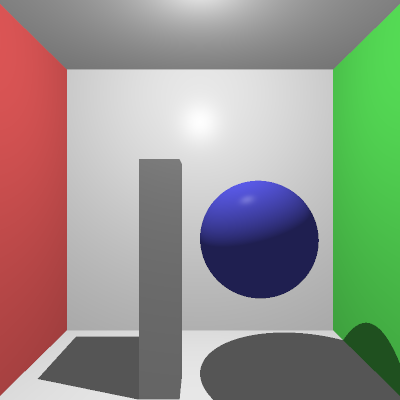
\includegraphics[width=0.65\textwidth]{teste_1.1_geometria.png}
  \caption{Geometria: Cornell Box com um pilar (caixa AABB) e uma esfera
           azul. A luz pontual central ilumina os objetos com sombreamento
           difuso. As normais da caixa e da esfera são computadas
           corretamente, confirmando o funcionamento do método dos planos
           paralelos e da interseção esfera-raio.}
\end{figure}

% ------------------------------------------------------------------
\subsection{Teste 1.2 — Modelo de Phong e Múltiplas Luzes}
% ------------------------------------------------------------------

\begin{figure}[H]
  \centering
  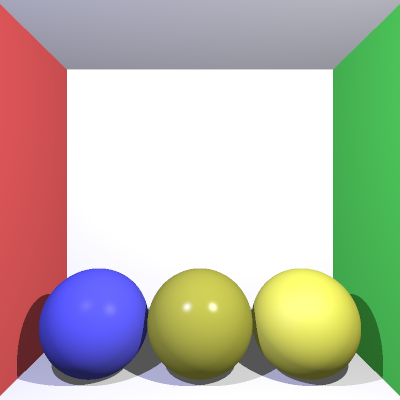
\includegraphics[width=0.65\textwidth]{teste_1.2_phong.png}
  \caption{Modelo de Phong com duas fontes de luz pontuais: uma branca
           (direita) e uma azulada (esquerda). As três esferas possuem
           materiais distintos: azul fosco (baixo especular), amarela
           brilhante (alto especular, shininess = 100) e amarela fosca
           (baixo especular, shininess = 5). Os realces especulares e a
           mistura de cores das duas luzes são claramente visíveis.}
\end{figure}

% ------------------------------------------------------------------
\subsection{Teste 1.3 — Sombras}
% ------------------------------------------------------------------

\begin{figure}[H]
  \centering
  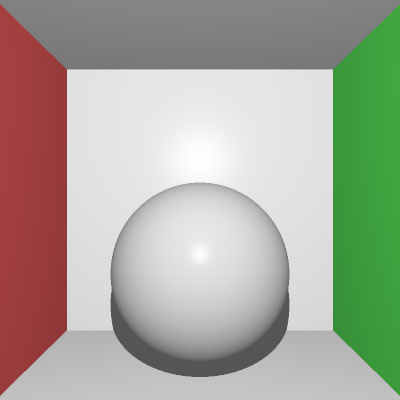
\includegraphics[width=0.65\textwidth]{teste_1.3_sombras.png}
  \caption{Sombra dura: a fonte de luz está posicionada atrás e acima
           da câmera. A esfera branca projeta sombra nítida sobre o chão
           e a parede do fundo. A ausência de \textit{shadow acne} na
           superfície da esfera confirma o deslocamento correto da origem
           do \textit{shadow ray}.}
\end{figure}

% ------------------------------------------------------------------
\subsection{Teste 1.4 — Antialiasing (Amostragem Uniforme)}
% ------------------------------------------------------------------

\begin{figure}[H]
  \centering
  \begin{subfigure}[b]{0.47\textwidth}
    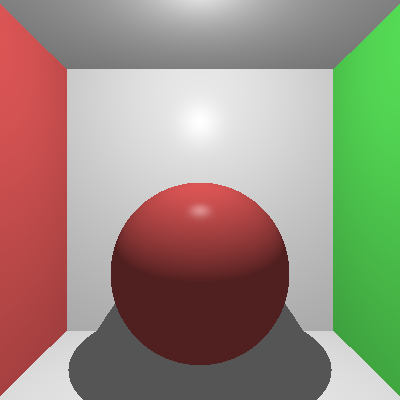
\includegraphics[width=\textwidth]{teste_1.4_aa_OFF.png}
    \caption{1 amostra por pixel (sem AA). Bordas serrilhadas visíveis.}
  \end{subfigure}
  \hfill
  \begin{subfigure}[b]{0.47\textwidth}
    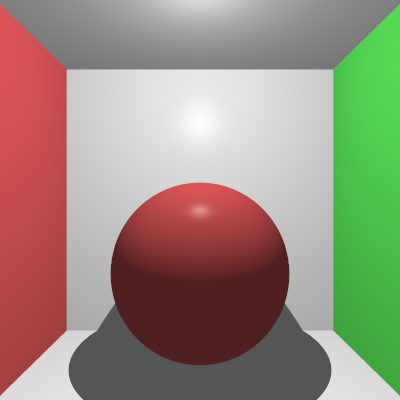
\includegraphics[width=\textwidth]{teste_1.4_aa_ON.png}
    \caption{16 amostras por pixel (grade 4$\times$4). Bordas suavizadas.}
  \end{subfigure}
  \caption{Comparação de antialiasing. Com 16 amostras em grade uniforme,
           o serrilhado nas bordas da esfera vermelha é significativamente
           reduzido, sem aumentar o viés espacial.}
\end{figure}

% ------------------------------------------------------------------
\subsection{Extensão 2.1 — Reflexão}
% ------------------------------------------------------------------

\begin{figure}[H]
  \centering
  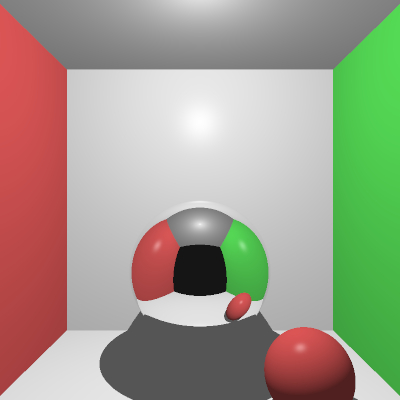
\includegraphics[width=0.65\textwidth]{teste_2.1_reflexao.png}
  \caption{Espelho com reflectividade $k_r = 0{,}95$ (material
           puramente reflexivo, sem componente difusa). A esfera espelhada
           ao centro reflete as paredes coloridas da Cornell Box e a esfera
           vermelha lateral. A reflexão é recursiva (até 5 níveis), permitindo
           múltiplos \textit{bounces}.}
\end{figure}

% ------------------------------------------------------------------
\subsection{Extensão 2.2 — Refração (Fresnel)}
% ------------------------------------------------------------------

\begin{figure}[H]
  \centering
  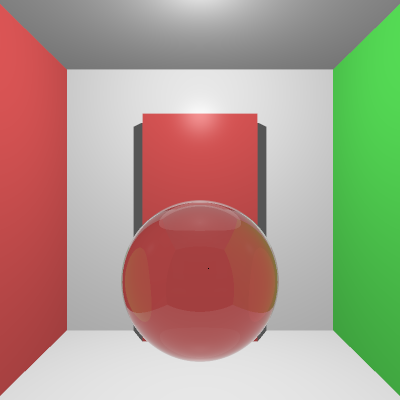
\includegraphics[width=0.65\textwidth]{teste_2.2_refracao.png}
  \caption{Esfera de vidro ($\eta = 1{,}5$) na frente de um pilar
           vermelho. As equações de Fresnel determinam a mistura entre
           reflexão (visível nas bordas, onde o ângulo de incidência é
           alto) e refração (interior da esfera, onde a imagem do fundo
           aparece invertida e deslocada). Quando o ângulo supera o
           ângulo crítico ($\theta_c = \arcsin(1/\eta) \approx 41{,}8°$),
           ocorre Reflexão Interna Total. O vidro não projeta sombra
           opaca, pois raios transparentes não bloqueiam a luz.}
\end{figure}

% ==================================================================
\section{Análise e Discussão}
% ==================================================================

\subsection{Desempenho}

O motor é implementado em Python puro com NumPy para operações vetoriais
por ponto, sem vetorização por imagem. Os tempos de renderização a
$400 \times 400$ pixels são apresentados na Tabela~\ref{tab:perf}.

\begin{table}[H]
  \centering
  \caption{Tempo de renderização por cenário (CPU, Python 3).}
  \label{tab:perf}
  \begin{tabular}{lcc}
    \toprule
    Cenário & Amostras/pixel & Tempo (s) \\
    \midrule
    1.1 Geometria        & 4  & $\approx 58$ \\
    1.2 Phong            & 4  & $\approx 80$ \\
    1.3 Sombras          & 4  & $\approx 48$ \\
    1.4a AA OFF          & 1  & $\approx 13$ \\
    1.4b AA ON           & 16 & $\approx 197$ \\
    2.1 Reflexão         & 4  & $\approx 56$ \\
    2.2 Refração         & 4  & $\approx 110$ \\
    \bottomrule
  \end{tabular}
\end{table}

O tempo da refração é aproximadamente o dobro do da reflexão, pois
cada interseção com vidro gera dois raios recursivos (refletido e
refratado), enquanto o espelho gera apenas um.

\subsection{Qualidade Visual}

\begin{itemize}
  \item \textbf{Phong:} o modelo captura bem a variação de brilho entre
        materiais com diferentes expoentes $\alpha$ e coeficientes $k_s$.
        Com duas luzes, surgem duplos realces especulares e mistura de
        cores nas regiões de penumbra parcial.

  \item \textbf{Sombras:} as sombras duras são fisicamente corretas para
        fontes pontuais. A ausência de \textit{shadow acne} valida o
        deslocamento de $10^{-4}$ na normal.

  \item \textbf{Antialiasing:} a grade uniforme $4\times4$ elimina o
        serrilhado visível com 1 amostra, especialmente nas bordas de
        alto contraste (esfera vermelha sobre fundo preto / paredes).

  \item \textbf{Reflexão:} a recursão com 5 níveis permite que o espelho
        mostre múltiplos reflexos das paredes coloridas da cena.

  \item \textbf{Refração:} as equações de Fresnel produzem o gradiente
        correto de reflexividade com o ângulo: bordas mais espelhadas,
        centro mais transparente. A imagem do fundo aparece invertida
        dentro da esfera de vidro, comportamento fisicamente esperado
        para $\eta = 1{,}5$.
\end{itemize}

% ==================================================================
\section{Conclusão}
% ==================================================================

O motor de traçado de raios implementado atende a todos os requisitos
básicos do projeto (geometria, iluminação Phong, sombras e amostragem
uniforme) e às extensões de reflexão (1{,}0 ponto) e refração com
equações de Fresnel completas (2{,}0 pontos). O resultado visual
demonstra o correto funcionamento de cada técnica, desde a interseção
geométrica até os efeitos ópticos de superfícies espelhadas e
dielétricas.

\end{document}
